% ----------------------------------------------------------------------
% 13eme Colloque National en Calcul des Structures
% ----------------------------------------------------------------------
% 15-19 mai 2017, Presqu'ile de Giens
% ----------------------------------------------------------------------
\documentclass{CSMA2017}
% ----------------------------------------------------------------------
\title{Méthodes de Newton non--lisses pour les problèmes de contact frottant dans les systèmes de multi--corps flexibles.}
% ----------------------------------------------------------------------
\author{V. Acary$^1$, M. Brémond$^1$, F. Dubois$^2$}
% ----------------------------------------------------------------------
\address{%
$^1$ INRIA. Grenoble, \{vincent.acary,maurice.bremond\}@inria.fr\\
$^2$ LMGC, Université de Montpellier, frederic.dubois@umontpellier.fr \\
}

% Mettre vos commandes personneles ici
% ----------------------------------------------------------------------
% Les commances \vect et \tens sont définies dans le fichier CSMA2017.cls


\def\RR{\nbR}
\def\NN{\nbN}
\def\nbR{\ensuremath{\mathrm{I\!R}}} % IR
\def\nbN{\ensuremath{\mathrm{I\!N}}} % IN

\def\n{{\hbox{\tiny{N}}}}
\def\t{{\hbox{\tiny{T}}}}

\def\tone{{\hbox{\tiny{T}}}_{\hbox{\tiny{1}}}}
\def\ttwo{{\hbox{\tiny{T}}}_{\hbox{\tiny{2}}}}

\def\nat{{\hbox{\sf \tiny{nat}}}}
\def\ac{{\hbox{\tiny{ac}}}}
\def\mjtwo{{\hbox{\tiny{mj}}}}
\usepackage{tikz}
\usepackage{xkeyval,tkz-base}
\usetikzlibrary{arrows}
\usetikzlibrary{calc}
\usepackage{mathtools}
\usepackage{subfig,float}
\usepackage{siunitx}
\usepackage{url}

\newcommand\red[1]{\textcolor{red}{#1}}
% ----------------------------------------------------------------------
\begin{document}
% ----------------------------------------------------------------------
\maketitle
% ----------------------------------------------------------------------

\begin{abstract}
Dans cette contribution, on se propose d'évaluer la performance des méthodes de Newton non--lisses dans le contexte des systèmes multi--corps flexibles (mécanismes, milieux granulaires ou milieux divisés) avec contact et frottement. Les méthodes itératives de type projection (Jacobi ou Gauss--Seidel projeté) sont généralement utilisées pour leurs propriétés de robustesse et de régularisation des systèmes fortement hyper--statiques. On montre que dans le cas des systèmes déformables, les méthodes de Newton permettent d'atteindre de grandes précisions à un coût beaucoup plus faible.

\keywords contact unilatéral, frottement de Coulomb, méthodes Newton non--lisses.
\end{abstract}

\section{Introduction}

Dans le contexte des systèmes multi--corps avec contact et frottement de Coulomb, le problème de contact frottant discret que l'on obtient à chaque pas de temps après une discrétisation temporelle, ou à chaque pas de chargement en quasi--statique, est généralement résolu par des méthodes itératives de type projection (Jacobi ou Gauss--Seidel projeté). 
%
Pour les systèmes de corps rigides, qui sont pour la plupart fortement hyperstatiques du fait d'un grand nombre de contacts en regard du nombre de degrés de liberté, les méthodes itératives jouissent de bonnes propriétés de robustesse. Elles permettent de converger de façon sure, mais lentement, vers une solution du problème même si les forces de réaction ne sont pas définies de manière unique. Il est connu que les méthodes de Newton non--lisses sont totalement inopérantes pour les systèmes rigides hyperstatiques~\cite{bertailsdescoubes:inria-00557706}. \marginpar{\red{Une autre citation?}}


Dans le cas de systèmes de corps flexibles, discrétisés par exemple par des éléments finis, il est facile de réduire ce degré d'hyperstaticité en augmentant le nombre de degrés de liberté du système. Un des objectifs est de réduire la dépendance des contraintes sur le système. Ceci peut par exemple se faire en raffinant les maillages dans les zones de  contact tout en contrôlant le nombre de points de contacts générés.
%
Dans cette contribution, on montre qu'il devient alors intéressant d'utiliser des méthodes de Newton non--lisses pour résoudre le problème discret, surtout si on veut atteindre des niveaux de précision relative supérieurs à $10^{-3}$.  Alors que les méthodes itératives de type projection continuent à converger lentement, les méthodes de Newton retrouvent leurs convergences quadratiques locales pour des systèmes fortement réguliers. Cela permet d'atteindre des niveaux de précisions arbitraires pour un coût de calcul bien moindre.


Dans ce travail\marginpar{\red{voir si on peut le faire. supprimer le paragraphe sinon}}, on essaye aussi de montrer qu'il peut être intéressant d'introduire un modèle de comportement élastique dans un système initialement rigide afin de profiter de l'efficacité numérique des méthodes de Newton. Dans des travaux antérieurs, M. Jean~\cite{Jean1999,Acary.Jean98} avait montré que l'introduction de l'élasticité permettait de réduire le degré d'hyperstaticité et d'améliorer sensiblement la qualité des solutions en termes de forces de réactions. En préférant des méthodes de Newton non--lisses, on améliore ainsi fortement le coût de calcul.


\paragraph{Formulation du problème.}
Considérons un nombre  $n_c\in \NN$ de points de contact tridimensionnel et un nombre   $n\in\NN$ de degrés de liberté du système discret. Pour chaque contact $\alpha$, les vitesses relatives locales au contact notées  $u^\alpha\in\RR^3$ et les réactions au contact notées $r^\alpha\in\RR^3$ (forces ou impulsions) sont décomposées dans un repère local au contact $({\sf N}^\alpha,{\sf T_1}^\alpha,{\sf T_2}^\alpha)$ tel que  $u^\alpha = u^\alpha_{\n} {\sf N}^\alpha +   u^{\alpha}_{\tone}{\sf T_1}^\alpha + u^{\alpha}_{\ttwo}{\sf T_2}^\alpha , u^\alpha_{\n} \in \RR, u^\alpha_{\t} = [u^{\alpha}_{\tone},u^{\alpha}_{\ttwo}]^\top \in \RR^2$ et  $r^\alpha = r^\alpha_{\n} {\sf N}^\alpha +   r^{\alpha}_{\tone}{\sf T_1}^\alpha + r^{\alpha}_{\ttwo}{\sf T_2}^\alpha  , r^\alpha_{\n} \in \RR, r^\alpha_{\t}=[r^{\alpha}_{\tone},r^{\alpha}_{\ttwo}]^\top \in \RR^2$. L'interstice au contact est noté $g_\n^\alpha$ (voir la figure~\ref{fig:local-frame}).

\begin{figure}
  \centering
  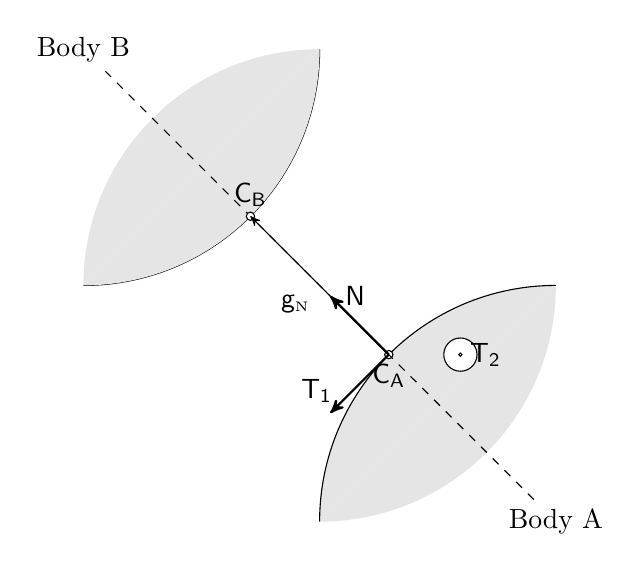
\begin{tikzpicture}[ scale=3,
      axis/.style={ ->, >=stealth'},
      normal/.style={ thick, ->, >=stealth'},
      important line/.style={very thick},
      dashed line/.style={dashed, thin},
      every node/.style={color=black},
      soldot/.style={only marks,mark=*},
      holdot/.style={fill=white,only marks,mark=*}
      ]
      % body
      \node (BodyA) at (1,-1) {Body A};
      \fill[gray!20] (1,0) arc (0:-90:1);
      \fill[gray!20] (1,0) arc (90:180:1);
      \draw (1,0) arc (90:180:1);

      \node (BodyB) at (-1,1) {Body B};
      \draw (0,1) arc (0:-90:1);
      \fill[gray!20] (0,1) arc (90:180:1);
      \fill[gray!20] (0,1) arc (0:-90:1);

      % local frame
      \def\nlength{0.35};
      \coordinate (CA)  at  ({1.0-sqrt(2)/2.0},{-1.0+sqrt(2)/2.0});
      \node[] at  (CA) [below] {$\sf C_A$};
      \draw[holdot]  (CA) circle(0.05em);
      \draw[normal] (CA) -- ($(CA)+({-\nlength*sqrt(2)/2.0},{+\nlength*sqrt(2)/2.0 })$) node [right] {$\,\sf N$};
      \draw[normal] (CA) -- ($(CA)+({-\nlength*sqrt(2)/2.0},{-\nlength*sqrt(2)/2.0 })$) node [above] {$\sf T_1\quad$};
      \draw[dashed line] (BodyA) -- (BodyB);
      \draw[holdot] ($(CA)+({\nlength*sqrt(3)/2.0},{0.0})$) circle(0.2em);
      \node at ($(CA)+({\nlength*sqrt(3)/2.0},{0.0})$) [right]{$\sf T_2$};
      \draw[soldot] ($(CA)+({\nlength*sqrt(3)/2.0},{0.0})$) circle(0.02em);

      \coordinate (CB)  at  ({-1.0+sqrt(2)/2.0},{1.0-sqrt(2)/2.0});
      \node at  (CB) [above] {$\sf C_B$};
      \draw[holdot]  (CB) circle(0.05em);

      \draw[axis] (CA) -- (CB) node[midway, below left ] {$\sf g_\n$} ;
      
      % \draw[axis] (0,-0.4) -- (0,0.4) node(yline)[right] {$\sgn(x)$};
      % % lines
      % \draw[important line] (-0.4,-0.3) -- (0.   ,-.3);
      % \draw[important line] (0.0,0.3) --(.4,.3)  ;
      % \coordinate (O) at (0.0, 0.05);
      % \draw[fill] (O) circle (0.03em);
      % \draw (0.0,0.05) node[right]{$a$};
      % \draw (0.0,0.3) node[left]{$1$};
      % \draw (0.0,-0.3) node[right]{$-1$};
      % \draw[holdot] (0.0,0.3) circle (0.03em);
      % \draw[holdot] (0.0,-.3) circle (0.03em);
    \end{tikzpicture}
\caption{Repère local au contact}
\label{fig:local-frame}
\end{figure}

Pour chaque contact, on définit le cône de Coulomb comme le cône du second ordre suivant:
\begin{equation}
  \label{eq:CoulombCone}
  K^\alpha = \{r^\alpha \in \RR^3 \mid \|r^\alpha_\t\| \leq \mu^\alpha r^\alpha_\n\}.
\end{equation}
où $\mu^\alpha$ est le coefficient de frottement du contact $\alpha$. Sous forme disjonctive, le contact unilatéral avec du frottement de Coulomb peut s'écrire en vitesse
\begin{equation}
  \label{eq:contact-disjunctive}
  \left\{\begin{array}{llr}
      r^\alpha = 0  &\text{ si } g^\alpha_{\n} > 0  & \text{(pas de  contact)}\\
      r^\alpha = 0,  u^\alpha_\n \geq 0   &\text{ si } g^\alpha_{\n} \leq 0 & \text{(décollage)} \\
      r^\alpha \in K^\alpha, u^\alpha =0 &\text{ si } g^\alpha_{\n} \leq 0 & \text{(adhérence)}  \\
      r^\alpha \in \partial K^\alpha,u^\alpha _\n=0,  \exists\,\beta > 0, u^\alpha_\t = -\beta r^\alpha_\t &\text{ si } g^\alpha_{\n} \leq 0 & \text{(glissement)}  \\
    \end{array}\right.
\end{equation}
En introduisant la vitesse relative locale modifiée $\hat u^\alpha = u^\alpha + \mu^\alpha \|u^\alpha_\t\| {\sf N}^\alpha$ due à~\cite{DeSaxce92}, le problème peut être reformulé de manière équivalente comme un problème de complémentarité du second ordre~\cite{DeSaxce92,Acary.ea_ZAMM2011} :
\begin{equation}
  \label{eq:contact-soccp}
  \left\{\begin{array}{ll}
      r^\alpha = 0  & \text{ si } g^\alpha_{\n} > 0  \\
      K^{\alpha,\star}\ni \hat u^\alpha \perp r^\alpha \in K^\alpha  & \text{ sinon. }\\
    \end{array}\right.
\end{equation}
Le cône $K^{\alpha,\star}$ est le cône dual de $K^\alpha$.

Suite à une discrétisation des équations du mouvement ou d'équilibre, et à une linéarisation si nécessaire, on peut relier les variables cinématiques $ {v} \in \RR^n$ aux efforts de contact par une relation linéaire, ce qui nous conduit à un  problème linéaire de complémentarité en cas de contact :
\begin{equation}\label{eq:soccp1-intro}
  \begin{array}{rcl}
    M v = {H} {r} + {f}, &
    u = H^\top v + w,  &
    \hat u = u + g(u) ,\\[1mm]
    &    K^\star \ni {\hat u} \perp r \in K,&
  \end{array}
\end{equation}
où $f\in \RR^n$ est homogène à des efforts, $K$ est le produit cartésien de cônes pour chaque contact, 
\begin{equation}
  \label{eq:CC}
  K = \prod_{\alpha=1\ldots n_c} K^{\alpha}  = \prod_{\alpha=1\ldots n_c} \{r^\alpha, \|r^\alpha_\t \| \leq \mu^\alpha |r^\alpha_\n| \}
\end{equation}
et $K^\star$ son dual. La fonction $g(u)$ est une fonction non--lisse définie par 
\begin{equation}
g(u) = [[\mu^\alpha  \|u^\alpha_\t\| {\sf N}^\alpha]^\top, \alpha = 1\ldots n_c]^\top\label{eq:gg}. 
\end{equation}
La matrice $M \in \RR^{n \times n}$ est le plus souvent définie positive. Nous nous placerons dans cet article dans les conditions d'existence de solution comme elles sont données dans~\cite{Klarbring.Pang1998,Acary.ea_ZAMM2011}.


\paragraph{Rang de la matrice $H$ et hyperstaticité.} 
Attardons nous un moment sur la matrice $H \in \RR^{n\times 3n_c} $ qui relie les efforts de contact $r$ aux efforts généralisés $R=H r$ et de façon duale les vitesses relatives au contact aux vitesses généralisées $u = H^\top v +w$ . Si le nombre de contacts est grand en rapport au nombre de degrés de liberté, disons $3 n_c > n$, la matrice $H$ ne peut pas être de rang plein par colonnes. Il en résulte une dépendance linéaire des efforts de contacts et une multiplicité de solutions. Dans le cas des systèmes de corps rigides, cette situation est liée a l'hyperstaticité du système. Elle est, de plus, la situation générique. Pensons par exemple à une table rigide à quatre pieds sur le sol. Naturellement, cette situation peut aussi arriver dans le cas $3 n_c \leq  n$ si des contraintes linéairement dépendantes sont appliquées aux corps. La réduction de rang de cette matrice influence fortement le comportement des méthodes numériques de résolution. 

Il en est de même si on cherche a résoudre le problème réduit aux variables locales au contact:
\begin{equation}\label{eq:soccp2-intro}
  \begin{array}{l}
    u = W r + q,  \\
    \hat u = u + g(u) \\
        K^\star \ni {\hat u} \perp r \in K,
  \end{array}
\end{equation}
avec $W \coloneqq H^\top M^{-1} H \in \RR^{3n_c\times 3n_c}$ la matrice de Delassus et $q \coloneqq w + H^\top M^{-1} f \in \RR^{3n_c}$. Dans ce cas, c'est la matrice $W$ qui n'est plus de rang plein et les mêmes problèmes sont constatés.

% \begin{itemize}
% \item Description du problème de frottement discret
% \item Problème de rang de H
% \item Objectifs du papier
%   \begin{enumerate}
%   \item Comparaison performance NSGS/NSN sur des déformables et des rigides.
%   \item Intérêt a passer en déformable pour ajouter des ddl.
%   \end{enumerate}
% \end{itemize}

\section{Méthodes numériques de résolution}
Rappelons brièvement les caractéristiques des méthodes utilisées dans cette étude. Pour plus de détails, on pourra consulter~\cite{Acary.Brogliato2008}.

\paragraph{Méthodes de Newton non--lisses.} 
Les méthodes  de Newton non--lisses sont basées sur une réécriture du problème sous la forme d'une équation $F(r)=0$, dont les racines sont les solutions du problème original. Parmi les exemples les plus connus de ces fonctions, on peut citer la fonction de P. Alart et A. Curnier~\cite{Alart.Curnier1991}:
\begin{equation}
  \label{eq:AC-1}
 F_\ac(r) \coloneqq  
  \left[
  \begin{array}{l} 
    r_\n - P_{\RR^{n_c}_+}(r_\n - \rho_\n  (Wr+q)_\n) = 0, \\
    r_\t - P_{D(\mu, (r_\n - \rho (Wr+q)_\n)_+)}(r_\t - \rho_\t (Wr+q)_\t   )=0
  \end{array}
  \right] =0,\quad \rho_\n>0, \rho_\t>0,
\end{equation}
avec le disque de frottement  $D(\mu,(r_{n})_+) = \prod_{\alpha=1\ldots n_c} \{ r_\t \in \RR^2 \mid  \|r_t\| \leq \mu (r_\n)_+  \}$. La fonction $P_X$ représente la projection euclidienne sur un convexe $X$. Une variante  est la fonction proposée par M. Jean et J.J. Moreau~\cite{Jean.Moreau1987} et utilisée dans une méthode de Newton dans~\cite{Christensen.Klarbring.ea1998}
\begin{equation}
  \label{eq:MJ-II}
    F_{\mjtwo}(r) \coloneqq \left[ \begin{array}{c}
    r_\n - P_{\RR^{n_c}_+}(r_\n - \rho_\n (W r +  q)_\n) \\
    r_\t - P_{D(\mu, (r_{\n})_+)}(r_\t - \rho_\t (Wr+q)_\t   ) 
  \end{array}\right] =0,\quad \rho_\n>0, \rho_\t>0.
\end{equation}
 D'autres fonctions de complémentarité peuvent aussi être utilisées comme la fonction naturelle:
\begin{equation}
  \label{eq:natural-II}
  F_\nat(r) \coloneqq   \left[
  \begin{array}{l} 
    r - P_{K}\left(r  - \rho (Wr+q + g(Wr+q))\right)
  \end{array}\right] 
  = 0, \quad \rho >0
\end{equation}
ou encore la fonction de Fisher-Burmeister. Partant de ces formulations, il convient ensuite de calculer(sélectionner) un élément régulier $\Phi$ du sous--différentiel de $F$ au point $r$, $\Phi(r) \in \partial F(r)$ et d'effectuer les itérations de Newton suivantes:
\begin{equation}
  \label{eq:NSN3}
  r_{k+1}  =  r_k -  \Phi^{-1}(r_k) (F(r_k)).
\end{equation}
Dans cet article, nous utilisons MUMPS~\cite{Amestoy.ea_PC2006,Amestoy.ea_SIAMMAA2001} pour la résolution des systèmes linéaires.

\paragraph{Méthodes de projection de type Gauss-Seidel.} 
La méthode de Gauss--Seidel avec projection est décrite en détail dans~\cite{Mitsopoulou.Doudoumis1987,Jourdan.Alart.ea98}. Elle consiste en une décomposition du problème contact par contact qui permet de calculer à l'itération $k$ les inconnues du contact $\alpha$ en résolvant le problème suivant 
\begin{equation}
  \label{eq:pgs-1}
  \begin{array}{c}
  u^{\alpha}_{k+1} = W^{\alpha\alpha} r^{\alpha}_{k+1} + \sum_{\beta < \alpha}W^{\alpha\beta} r^{\beta}_{k+1} + \sum_{\beta > \alpha}W^{\alpha\beta} r^{\beta}_{k} +  q^\alpha,\\[1mm] 
  \hat u^{\alpha}_{k+1} =u^{\alpha}_{k+1} + g(u^{\alpha}_{k+1}), \\[1mm]
   K^{\alpha,\star} \ni {\hat u^{\alpha}_{k+1}} \perp r^{\alpha}_{k+1} \in K^\alpha.
 \end{array}
\end{equation}
La résolution du problème local au contact~(\ref{eq:pgs-1}) peut se faire de manière analytique, ou en utilisant une autre méthode numérique. Dans cet article, on utilisera localement une méthode de Newton non--lisse comme décrite ci--dessus ou des itérations de points fixe de $F_\nat(r)-r$.

\paragraph{Nomenclature.} 
Dans la suite, les méthodes utilisées sont nommées comme dans la Table~\ref{tab:nomenclature}.
\begin{table}
  \centering
  \begin{tabular}{ll}
    \hline
    {\sf\small NSN-AC-NLS} & Méthode de Newton non--lisse utilisant~(\ref{eq:AC-1}) sans recherche linéaire \\
    {\sf\small NSN-JM-NLS} & Méthode de Newton non--lisse utilisant~(\ref{eq:MJ-II}) sans recherche linéaire \\
    {\sf\small NSN-NM-NLS} & Méthode de Newton non--lisse utilisant~(\ref{eq:natural-II}) sans recherche linéaire \\
    {\sf\small NSN-AC-NLS-HYBRID} & Méthode {\sf\small NSN-AC-NLS} avec  un pré--conditionnement par $100$ itérations de {\sf\small NSGS-AC} \\
    {\sf\small NSGS-AC} & Méthode de Gauss Seidel avec {\sf\small NSN-AC-NLS} pour méthode locale\\
    {\sf\small  NSGS-FP-VI-UPK} & Méthode de Gauss Seidel avec itérations locales de points fixe de $F_\nat(r)-r$\\
    \hline 
  \end{tabular}
  \caption{Nomenclature des méthodes utilisées}
  \label{tab:nomenclature}
\end{table}

\paragraph{Mesure d'erreur.} 
Afin de comparer la convergence des méthodes, nous utilisons un critère d'arrêt à une précision utilisateur $\epsilon$ basée sur la fonction naturelle pour les problèmes de complémentarité du second ordre:
\begin{equation}
  \label{eq:stopping-criteria-full}
  \displaystyle\frac{\|F_\nat(r)\|}{\|q\|} < \epsilon,
\end{equation}
en supposant que le problème n'est pas dégénéré($\|q\| \neq 0$). \\
%
Cette mesure d'erreur est justifiée plus amplement dans \cite{Facchinei.Pang2003}. Dans le cas des méthodes itératives de projection, le coût de calcul de $F_\nat(r)$ est élevé par rapport à une itération. Nous utilisons un critère d'arrêt du type 
\begin{equation}
  \label{eq:stopping-criteria-light}
  \displaystyle\frac{\|r_{k+1}- r_{k}\|}{\|r_{k+1}\|} < \tau,
\end{equation}
où $\tau$ est adapté en ligne pour atteindre le critère~(\ref{eq:stopping-criteria-full}).

\paragraph{Profil de performance.} 
Pour évaluer l'efficacité d'une méthode par rapport à une autre, nous utilisons les profils de performance comme ils sont proposés dans~\cite{DolanMore_MP2002}. Considérons un ensemble $\mathcal P$ de $n_p$ problèmes et $\mathcal S$  de $n_s$ méthodes de résolutions. Pour chaque problème $p\in \mathcal P$ et chaque méthode $s \in \mathcal S$, on définit un critère de performance $t_{p,s}$. Dans notre cas, il s'agira du nombre d'opérations flottantes pour atteindre une précision donnée. De plus, si la précision n'est pas atteinte au bout d'un temps de calcul maximum par problème ($1000\si{\second}$), le critère est égal à $+\infty$. On définit le rapport de performance par:  
\begin{equation}
 r_{p, s} = \frac{t_{p,s}}{\text{min}\, \{t_{p,s}, \, \, s \in S\}} \, .
\end{equation}
Enfin on définit la probabilité  $\rho_s(\tau)$ pour une méthode $s \in S$ que le rapport de perfomance $r_{p, s}$ soit en dessous d'une valeur $\tau \in \mathbb R$ :
\begin{equation}
 \rho_s(\tau) = \frac{1}{n_p} \text{size} \{p \in P, \, \, r_{p, s} \leq \tau\} \geq 1.
\end{equation}
On peut remarquer que $\rho_s(1)$ représente la probabilité que la méthode $s$ soit la meilleure par rapport aux autres méthodes. La valeur $\rho_s(\tau)$ pour $\tau$ grand caractérise la capacité de la méthode à résoudre un grand nombre de problème en temps long. Les fonctions $\tau \rightarrow \rho_s(\tau) $ sont des fonctions croissantes dont  on tracera les graphes appelés profils de performance pour une plage de $\tau$. 



\section{Comparaison sur des solides élastiques}

\paragraph{La murette.}
L'exemple choisi pour illustrer le comportement des solveurs est la modélisation d'une maçonnerie en appareil régulier composée de 12 blocs et soumise à un chargement de cisaillement illustrée à la figure~\ref{fig:LowWall_FEM}. Les blocs sont maillés par des éléments finis linéaires avec un comportement élastique linéaire ($\rho= \num{2000}\si{\kilogram\per\cubic\metre}, E=\num{2.2e+9}\si{\pascal} ,\nu = 0.2$). L'interface entre les blocs est modélisée par du frottement de Coulomb avec du contact unilatéral.  Le coefficient de frottement entre les blocs est de $0.83$ et entre les blocs et les supports de $0.53$. Le support du bas est fixe. Sur le support du haut on applique un effort  maximum de compression de $30000 \si{\newton}$ et une vitesse tangente de cisaillement de $\num{1e-3}\si{\meter\per\second}$.
\marginpar{\red{verifier la description. nombre et type d'éléments}} Le nombre de points de contact est $2064$ et le nombre de degré de liberté est $7212$. La matrice $H$ est de rang plein.
\begin{figure}[htbp]
  \centering
  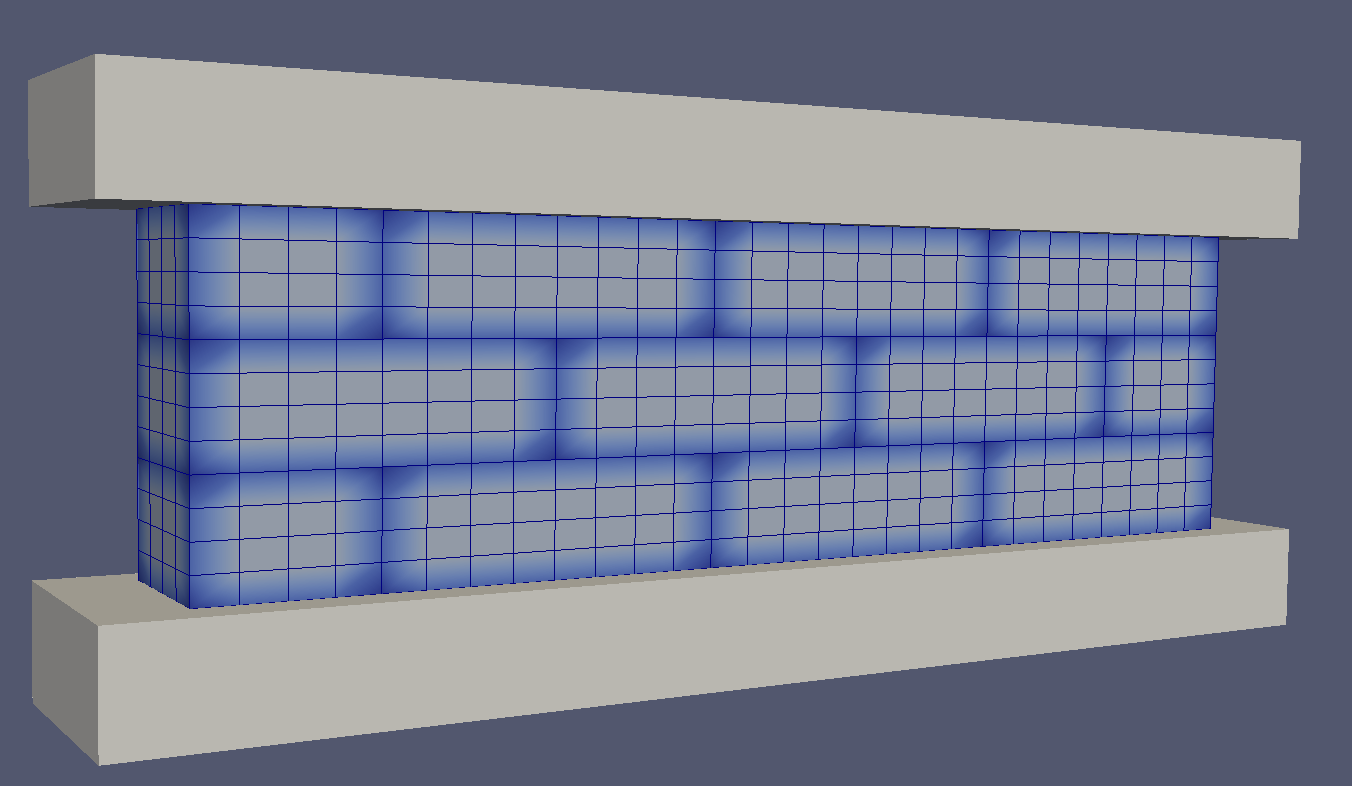
\includegraphics[height=0.2\textheight]{./figure/LowWall_FEM.png}
  \caption{Une murette}
  \label{fig:LowWall_FEM}
\end{figure}

\paragraph{Génération d'exemples par simulation et logiciels.}
Le système est modélisé et simulé par le logiciel LMGC90. A chaque pas de temps, on résout le problème discret de frottement avec Siconos/numerics et on exporte le problème discret à résoudre dans un fichier au format FClib. De cette collection d'exemples, on extrait  50 problèmes de difficulté graduée pour la méthode de Newton non--lisse.

 LMGC90~\cite{dubois2003lmgc90} est une plateforme de d{\'e}veloppement d{\'e}di{\'e}e {\`a} la mod{\'e}lisation des probl{\`e}mes d’interaction. L'implantation des méthodes de résolution est faite dans Siconos~\cite{siconos} qui est un logiciel open--source de modélisation et de simulation des systèmes dynamiques non lisse.  Enfin FCLib~\cite{acary:hal-00945820} est un format et une collection ouverte de problèmes de frottement qui permet de comparer des méthodes de résolution sur une large base d'exemples.

\paragraph{Résultats.}
Sur la figure~\ref{fig:LowWall_FEM.simple}, on représente les profils de performance des méthodes de résolution pour des précisions différentes. 

Pour une précision relativement faible de $10^{-2}$, les performances des méthodes sont très proches. Les méthodes de Newton non lisses  {\sf\small NSN-AC-NLS}, {\sf\small NSN-JM-NLS} et {\sf\small NSN-AC-NLS-HYBRID} sont légèrement meilleures que {\sf\small NSGS-AC} et {\sf\small NSGS-FP-VI-UPK}. La méthode {\sf\small NSN-AC-NLS-HYBRID} qui utilise un pré--conditionnement apparaît comme étant la plus performante ce qui est logique puisque les méthodes de projection permettent de trouver une solution grossière plus rapidement. La méthode {\sf\small NSN-NM-NLS} est la moins performante.

Pour une précision de $10^{-3}$, toutes les méthodes de Newton non--lisses sont plus performantes. Elles sont les plus rapides et ne posent pas de problème de robustesse. La méthode {\sf\small NSN-NM-NLS} est la moins performante des méthodes de Newton. On peut noter que la méthode {\sf\small NSN-AC-NLS-HYBRID}  est la plus performante et qu'elle est en moyenne 4 fois plus performante que la méthode  {\sf\small NSGS-AC}. 

Pour une précision de  $10^{-4}$ et $10^{-6}$, cette tendance s'accentue avec des méthodes de Newton qui sont en moyenne $20$ fois et respectivement $40$ fois plus performantes que les méthodes itératives de projection. Un zoom sur les méthodes de Newton montre que leur performance relative reste inchangée. Par contre, la méthode de {\sf\small NSGS-FP-VI-UPK} devient plus performante que la méthode de {\sf\small NSGS-AC} pour une précision de $10^{-6}$.

% \begin{figure}
%   \centering
%   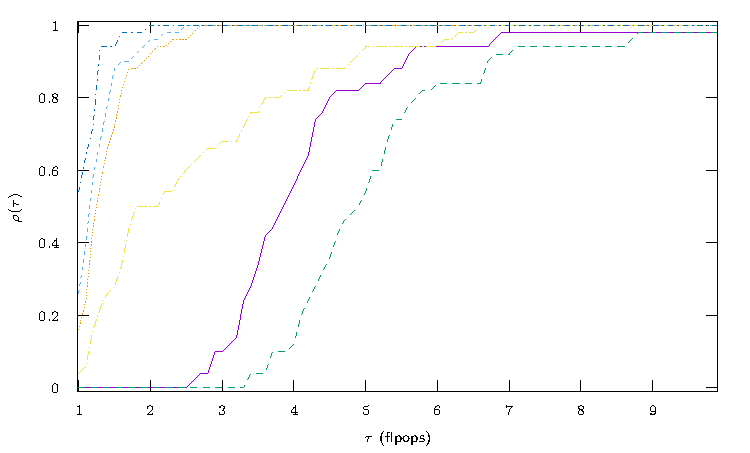
\includegraphics{figure/LowWall_FEM.1e-3.with_guess/simple/profile-LMGC_LowWall_FEM.pdf}
%   \includegraphics{figure/LowWall_FEM.1e-3.with_guess/simple/profile-LMGC_LowWall_FEM_legend.pdf}
%   \caption{Comparaison entre le solveur NSGS-AC et NSN-AC pour une précision de $10^{-3}$}
%   \label{fig:LowWall_FEM.1e-3.simple}
% \end{figure}
% \begin{figure}
%   \centering
%   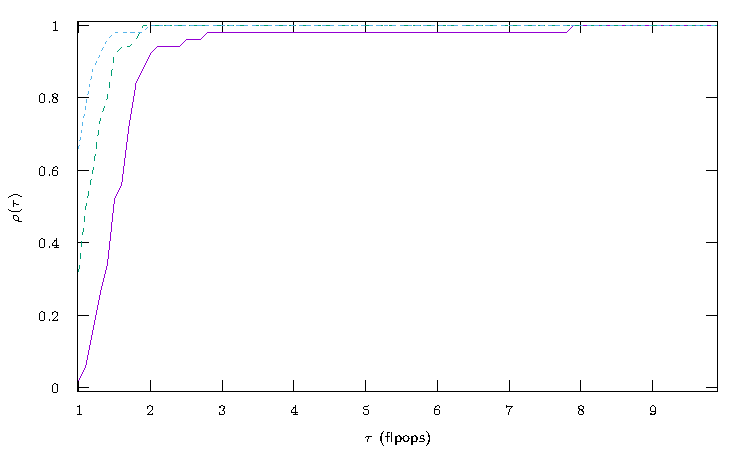
\includegraphics{figure/LowWall_FEM.1e-4.with_guess/simple/profile-LMGC_LowWall_FEM.pdf}
%   \includegraphics{figure/LowWall_FEM.1e-4.with_guess/simple/profile-LMGC_LowWall_FEM_legend.pdf}
%   \caption{Comparaison entre le solveur NSGS-AC et NSN-AC pour une précision de $10^{-4}$}
%   \label{fig:LowWall_FEM.1e-4.simple}
% \end{figure}
% \begin{figure}
%   \centering
%   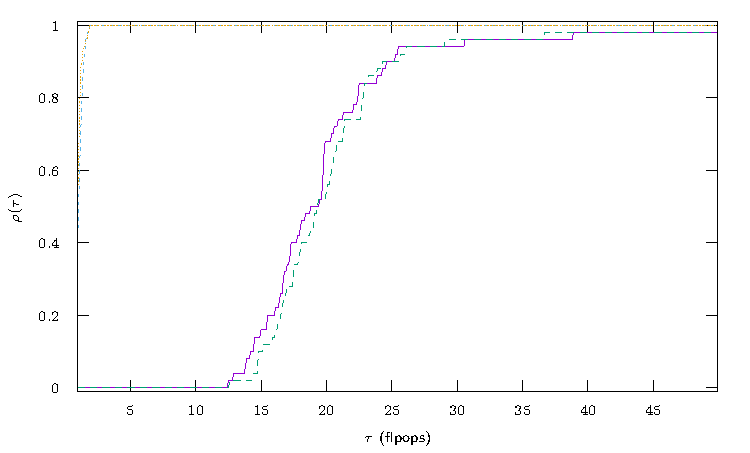
\includegraphics{figure/LowWall_FEM.1e-6.with_guess/simple/profile-LMGC_LowWall_FEM.pdf}
%   \includegraphics{figure/LowWall_FEM.1e-6.with_guess/simple/profile-LMGC_LowWall_FEM_legend.pdf}
%   \caption{Comparaison entre le solveur NSGS-AC et NSN-AC pour une précision de $10^{-6}$}
%   \label{fig:LowWall_FEM.1e-6.simple}
% \end{figure}
% \begin{figure}
%   \centering
%   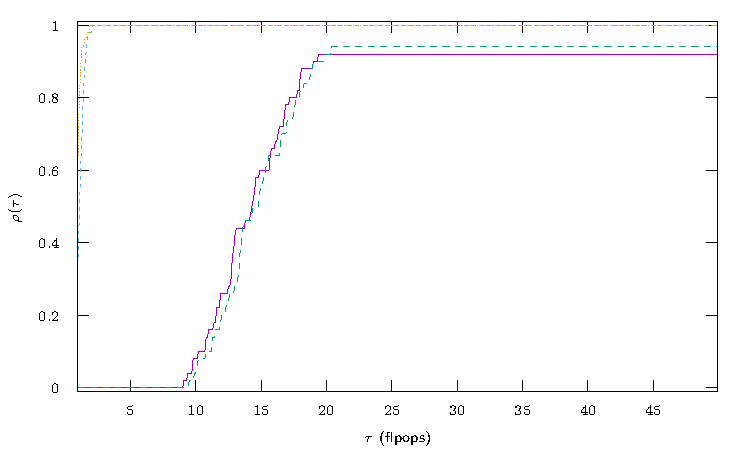
\includegraphics{figure/LowWall_FEM.1e-8.with_guess/simple/profile-LMGC_LowWall_FEM.pdf}
%   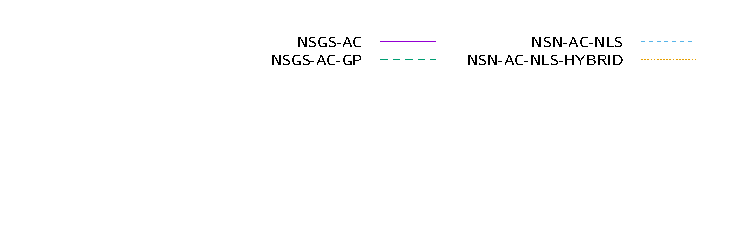
\includegraphics{figure/LowWall_FEM.1e-8.with_guess/simple/profile-LMGC_LowWall_FEM_legend.pdf}
%   \caption{Comparaison entre le solveur NSGS-AC et NSN-AC pour une précision de $10^{-8}$}
%   \label{fig:LowWall_FEM.1e-8.simple}
% \end{figure}

\begin{figure}[htbp]
  \centering 
  \subfloat[précision $\epsilon = 10^{-2}$]{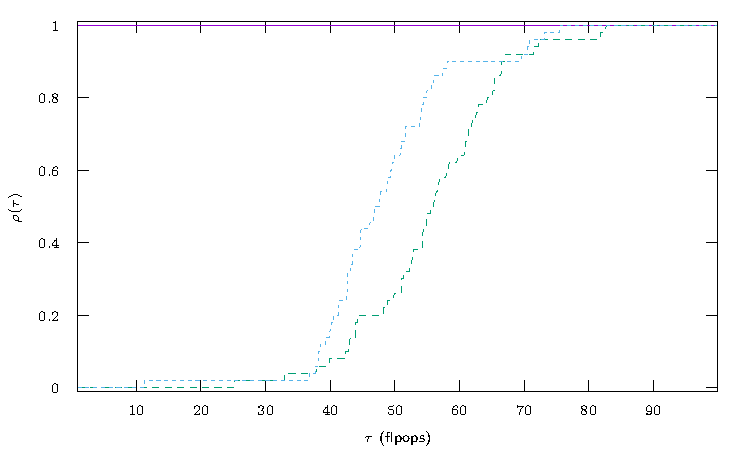
\includegraphics[width=0.49\textwidth]{figure/LowWall_FEM.1e-2.with_guess/simple/profile-LMGC_LowWall_FEM.pdf}\label{fig:LowWall_FEM.1e-2.simple}}
   \subfloat[précision $\epsilon = 10^{-3}$]{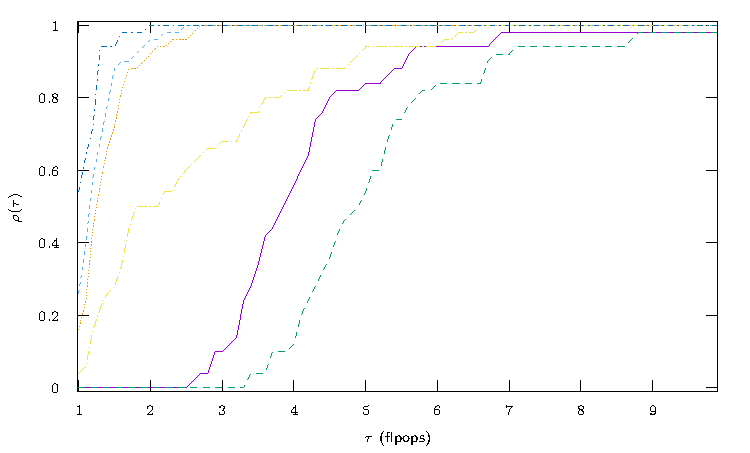
\includegraphics[width=0.49\textwidth]{figure/LowWall_FEM.1e-3.with_guess/simple/profile-LMGC_LowWall_FEM.pdf}\label{fig:LowWall_FEM.1e-3.simple}}\\
   \subfloat[précision $\epsilon =  10^{-4}$]{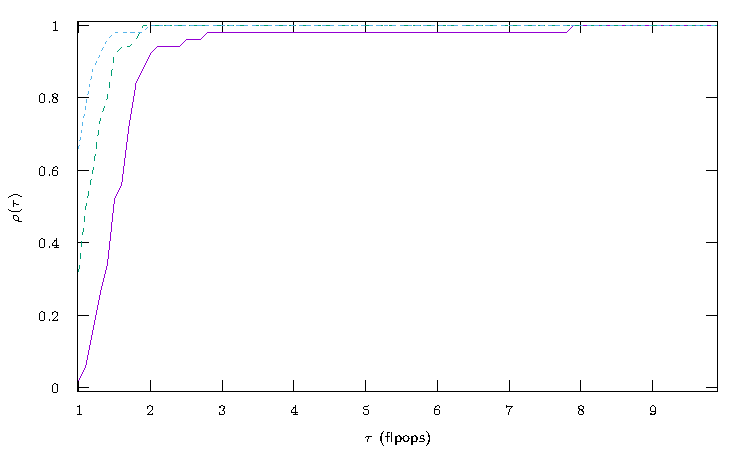
\includegraphics[width=0.49\textwidth]{figure/LowWall_FEM.1e-4.with_guess/simple/profile-LMGC_LowWall_FEM.pdf}\label{fig:LowWall_FEM.1e-4.simple}}
   \subfloat[précision $\epsilon = 10^{-6}$]{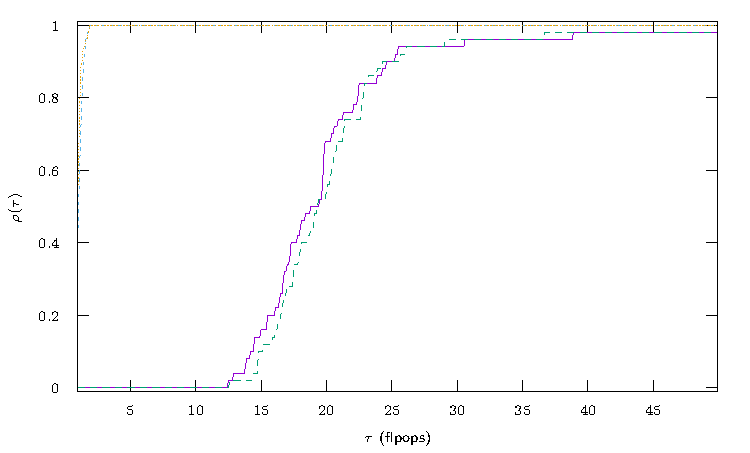
\includegraphics[width=0.49\textwidth]{figure/LowWall_FEM.1e-6.with_guess/simple/profile-LMGC_LowWall_FEM.pdf}\label{fig:LowWall_FEM.1e-6.simple}}\\
   % \subfloat[précision $\epsilon = 10^{-8}$]{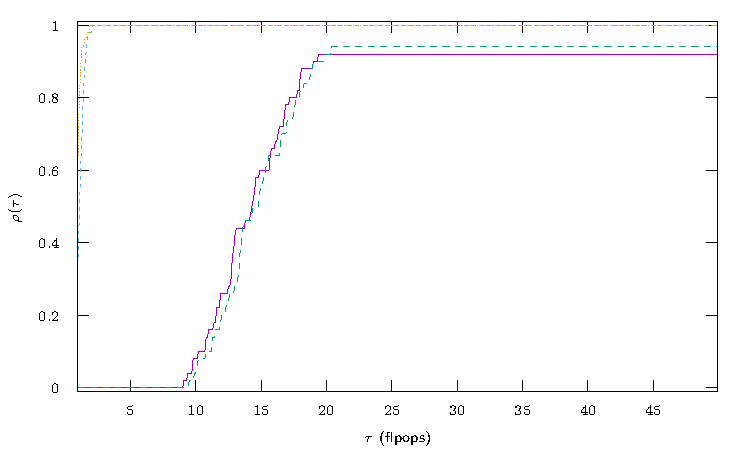
\includegraphics[width=0.49\textwidth]{figure/LowWall_FEM.1e-8.with_guess/simple/profile-LMGC_LowWall_FEM.pdf}\label{fig:LowWall_FEM.1e-8.simple}}\\
   \includegraphics{figure/LowWall_FEM.1e-2.with_guess/simple/profile-LMGC_LowWall_FEM_legend.pdf}
  \caption{Comparaison entre les méthodes itératives de type projection et les méthodes de Newton non--lisses pour différentes précisions.}
  \label{fig:LowWall_FEM.simple}
\end{figure}


% \begin{figure}
%   \centering
%   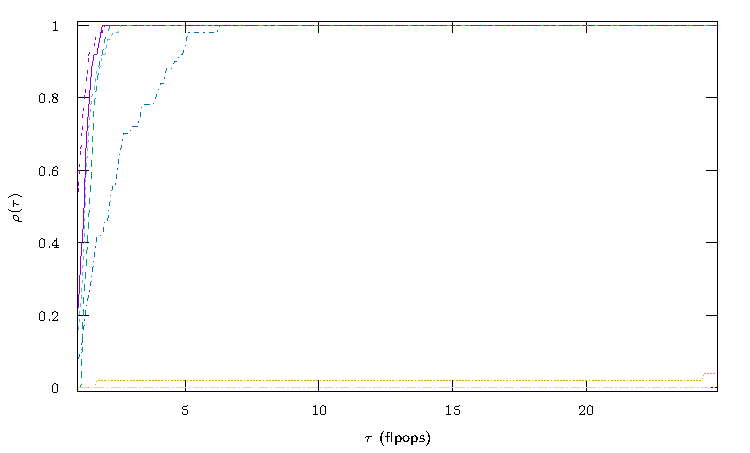
\includegraphics{figure/LowWall_FEM.1e-4.with_guess/nsn_nls/profile-LMGC_LowWall_FEM.pdf}
%   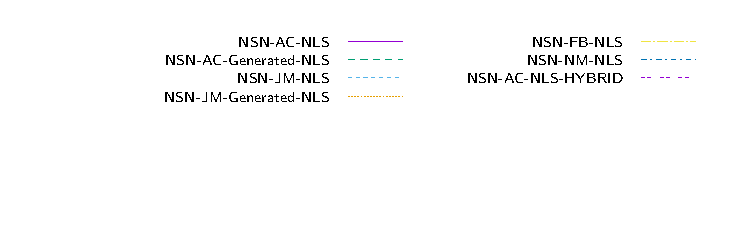
\includegraphics{figure/LowWall_FEM.1e-4.with_guess/nsn_nls/profile-LMGC_LowWall_FEM_legend.pdf}
%   \caption{Comparaison des solveurs NSN-*-NLS pour une précision de $10^{-4}$}
%   \label{fig:LowWall_FEM.1e-4.nsn_nls}
% \end{figure}
% \begin{figure}
%   \centering
%   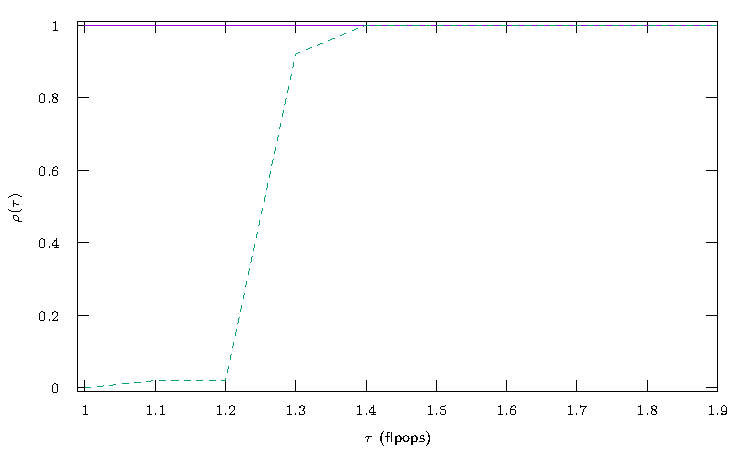
\includegraphics{figure/LowWall_FEM.1e-4.with_guess/nsgs/profile-LMGC_LowWall_FEM.pdf}
%   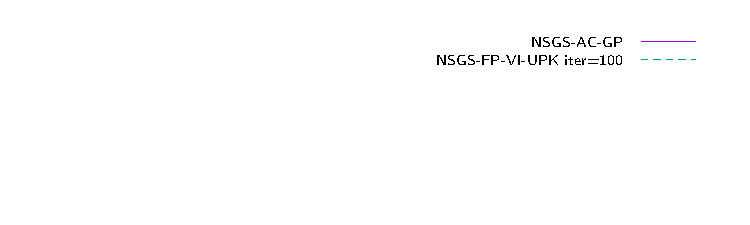
\includegraphics{figure/LowWall_FEM.1e-4.with_guess/nsgs/profile-LMGC_LowWall_FEM_legend.pdf}
%   \caption{Comparaison des solveurs NSGS pour une précision de $10^{-4}$}
%   \label{fig:LowWall_FEM.1e-4.nsgs}
% \end{figure}



% \section{Comparaison sur des solides rigides}

% \section{Utilisation des solides élastiques pour améliorer la convergence}

\section{Conclusion}

En conclusion, on peut observer que 
\begin{itemize}
\item Pour des précisions relativement élevées (au delà de $10^{-4}$), les méthodes de Newton lisses sont beaucoup plus performantes pour des systèmes multi--corps flexibles.
\item La méthode {\sf\small NSN-AC-NLS-HYBRID} est la méthode la plus performante des méthodes de Newton. Le pré--conditionnement permet d'accélérer la convergence des premières itérations de Newton.

\item Les méthodes itératives de projection restent intéressantes pour des précisions faibles, mais elles ne permettent pas d'atteindre une précision élevée pour un coût raisonnable.
\end{itemize}
\ \\
Les perspectives à ce travail sont les suivantes:
\begin{itemize}
\item évaluer l'intérêt de passer à un modèle déformable pour accélérer les calculs de systèmes multi--corps rigides. \marginpar{\red{c'était dans l'intro mais on a pas eu le temps ==> reprendre l'intro} }
\item intégrer le comportement non--linéaire de corps dans les méthodes de Newton non--lisse. Ceci permettrait d'éviter une boucle externe de Newton.
\item utiliser les potentialités massivement parallèles des librairies de calculs de grands systèmes linéaires comme MUMPS qui sont utilisées dans les méthodes de Newton. Cela pourrait fournir une alternative aux méthodes de Gauss--Seidel distribuées.
\end{itemize}



%\subsection{Références bibliographiques}

% Les références sont à insérer en fin de document, numérotées par ordre alphabétique des auteurs. Trois exemples de références sont proposés : un article \cite{article} et un acte \cite{acte} et un livre  \cite{livre}.


\bibstyle{plain}
\bibliography{biblio}

% % ----------------------------------------------------------------------
% \begin{thebibliography}{1}
% % ----------------------------------------------------------------------
% \bibitem{article}
% P. Auteur, D. Auteur, T. Auteur. \emph{Titre de l'article}, Revue, Éditeur, page1-pageN, Année. 
% \bibitem{acte} P. Auteur. \emph{Titre de l'acte}, Titre de l'ouvrage, Éditeur, page1-pageN, Année.
% \bibitem{livre} P. Auteur, D. Auteur. \emph{Titre de l'ouvrage}, Éditeur, Année. 

% % ----------------------------------------------------------------------
% \end{thebibliography}
% % ----------------------------------------------------------------------

% ----------------------------------------------------------------------
\end{document}
% ----------------------------------------------------------------------
